% !TEX root = ../../fyp.tex
\documentclass[../../fyp.tex]{subfiles}

\begin{document}
Word embeddings seek to tackle the non-trivial task of accurately capturing as much of the intricate details that are inherent in language, as possible. To model the intricacies of a word within the context of a particular language corpus, sophisticated models are employed to construct continuous and real-valued vectors for each word. The resulting vectors are commonly referred to as word embeddings, and are meant to be numerical representations of contexts in which each word is used  \cite{bengio2003} \cite{mikolov2013} \cite{pennington} \cite{tang}.

By first learning a continuous word vector embedding from data \cite{bengio2003} \cite{mikolov2013} \cite{pennington}, most approaches can take advantage of the principle of \textit{compositionality} \cite{frege1892} to obtain a sentence or indeed a document level representation for a myriad of downstream NLP tasks, including sentiment analysis.

Two of the most prominent word embedding models that are currently employed in many NLP tasks are \textit{word2vec} \cite{mikolov2013} and \textit{GloVe} \cite{pennington}. More recently, an extension on the former, termed \textit{fasttext} \cite{bojanowski2017} is also garnering considerable attention within the field, distinguishing itself from the other models mentioned through the use of sub-word information.

% \subsection{Word Embedding Methods}
The two principal methods for learning such distributional word representations are count-based and prediction-based, each with their own strengths and shortcomings, and neither being clearly superior to the other in every aspect. The former typically involves performing dimensionality reduction on a co-occurrence count matrix, whereas the latter is derives word representations from learning to correctly predict words or contexts within a bounded, moving, window \cite{pennington}.

Both methods provide a powerful means of autonomously extracting expressive and meaningful features from a wealth of text to the degree that would be unfeasible through manual means alone due to the staggering complexity inherent in language itself as well as the sheer volume of data that is being constantly made available through various online platforms.

One of the benefits that is had from constructing a vector space with distributional representations of words is the ability to model features such as similarity between the constituent words and subsequently group words with similar meanings which expands a downstream model's comprehension of a language \cite{mikolov2013b}.

%TODO: indicate what word-analogy tasks are  
Matrix factorization methods, such as Latent Semantic Analysis (LSA) \cite{deerwester1990} as cited in Pennington et al. \cite{pennington}, attempt to extrapolate significant statistical information pertaining to a specific corpus, from decomposed matrices that are typically obtained through low-rank approximations. Although techniques such as LSA do this effectively, Pennington et al. \cite{pennington} note a lackluster performance in word-analogy tasks, which ultimately depend, in large part, on accurately capturing the aforementioned similarity between words in the vector space.

Models trained using matrix factorization methods are efficient at exploiting statistical information, and are typically easier to parallelize albeit at a higher initial memory investment involved in storing the co-occurrence matrix \cite{pennington}. Mikolov et al. \cite{mikolov2013} work on the assumption that more related words will tend to appear closer to each other than not, making window-based approaches ideal for word analogy tasks that benefit from accurate word-similarity modelling.

Since predictive methods rely on a bounded context window of some specified width when making predictions a trivial disadvantage that presents itself immediately with this approach is the limited capacity to efficiently exploit redundancy in the data on at a macro-scale. This is due to the fact that these methods operate on the level of their current context window as opposed to the document as a whole \cite{pennington}.

\subsection{Word2Vec}
\citet{mikolov2013} note that the tendency in the field of NLP was to regard words in an isolated fashion as opposed to considering each word within the scope of a distributed space where more in-depth information could be encoded regarding the relationship between words. Models, such as the popular n-gram model where prevalent in the literature due to their simplicity and effectiveness. They note that these methods had largely peaked as unlike distributed representations, they were limited in their capacity to model relationships, such as similarity, between words.

There was a need for more sophisticated, and scalable, techniques to address the bottleneck that was presenting itself in the lack of accurately labelled data that was being made available for training models in fields such as Automatic Speech Recognition (ASR) and machine translation. As these models emerged to tackle increasingly large data sets, simpler models, such as the aforementioned n-gram model, were consistently outperformed by neural networks using distributed representations of words in the form of word embeddings. Moreover, neural networks were shown to capture the linear relationships between words more accurately than previous methods that used LSA, while maintaining a higher level of scalability when compared to LDA \cite{mikolov2013}.

Some of the initial work making use of neural networks to learn word embeddings include \cite{collobert2008}, later refined in \citet{collobert2011}. Their approach consisted of a feedforward neural network tasked with predicting the correct word within a context window of five words including the target word itself.

Mikolov et al. \cite{mikolov2013} introduced the Continuous Skip-gram and the Continuous Bag-Of-Words (CBOW) models in an effort to extract word embeddings from large corpora. As illustrated in figure \ref{fig:cbow_vs_skipgram}, the former aims to learn an adequate representation of a word by training to predict the words that are most likely to surround it while, inversely, the latter was trained to predict a specific word given its context, both using a feed-forward neural network with the non-linear hidden layer removed.

\begin{figure}[!ht]
	\centering
	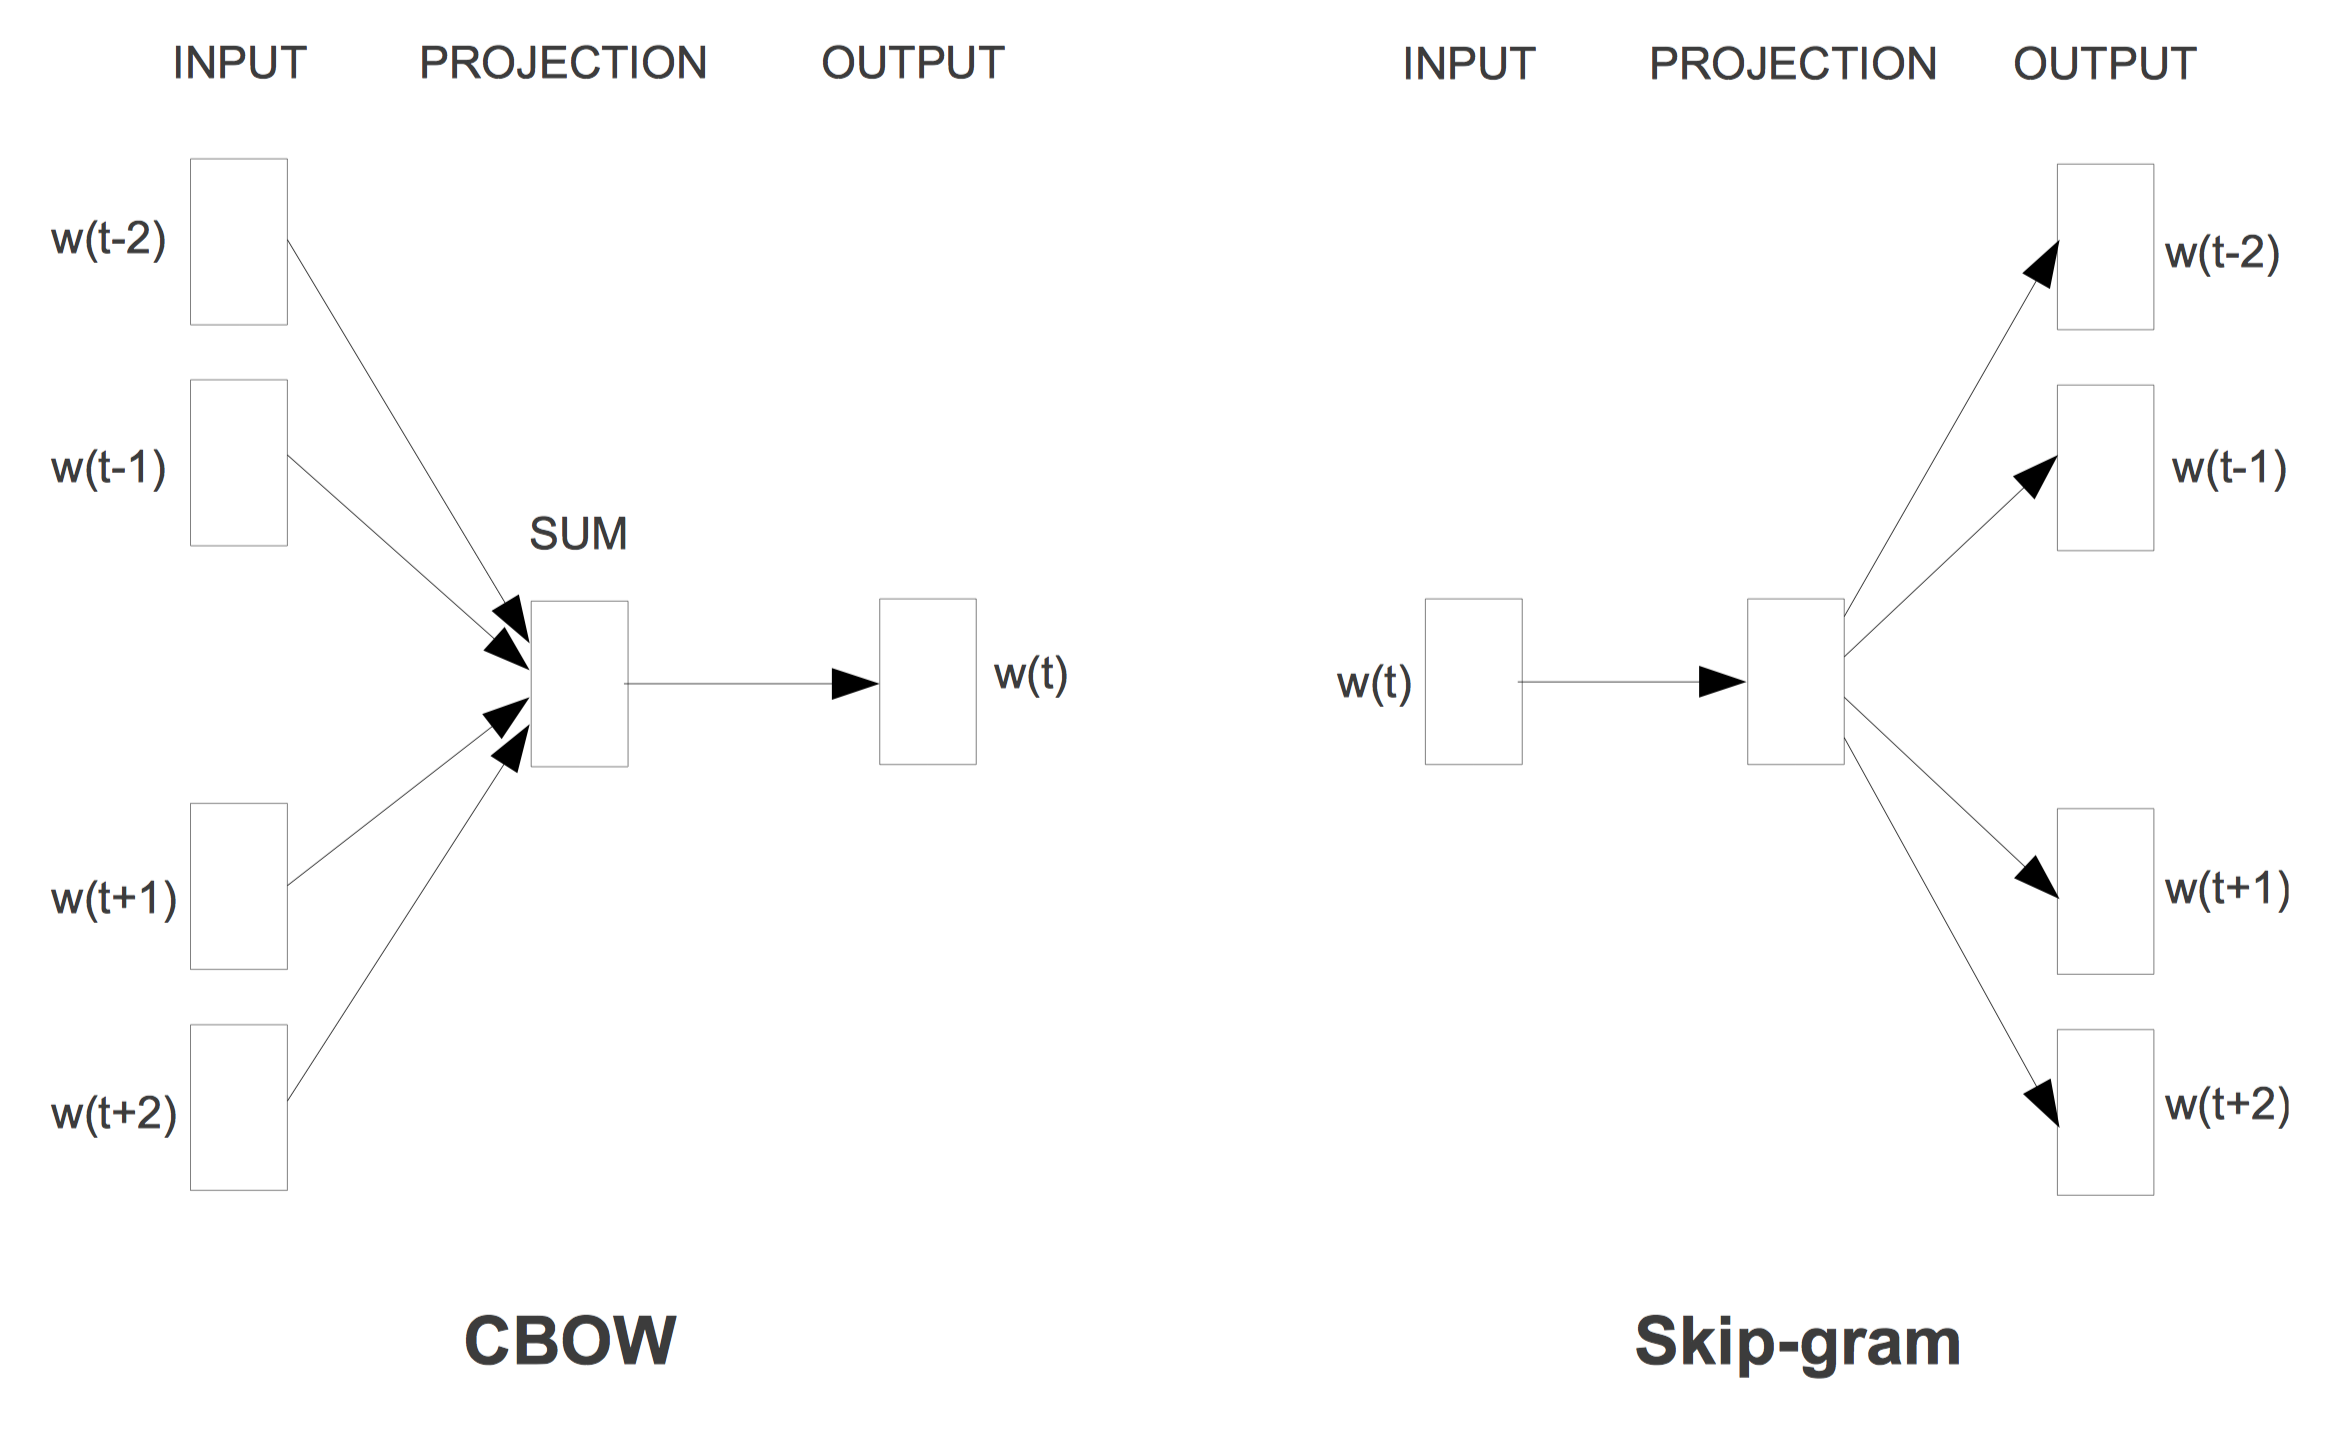
\includegraphics[width=0.7\textwidth]{cbow_vs_skipgram.png}
	\caption{The differences between the model architectures proposed by Mikolov in \cite{mikolov2013}. The Continuous Bag-Of-Words (CBOW) approach predicts a word from its context and, conversely, the skip-gram model predicts the context from a word \cite{mikolov2013b}.}
	\label{fig:cbow_vs_skipgram}
\end{figure}

Their work brought about a novel evaluation strategy which measures the expressive capacity of a word vector space through complex multi-dimensional comparisons that went over and above previous scalar metrics that were typically limited to the distance or angle between word vectors. As evidence of the level of sophistication obtained in the representations that were generated using the \textit{skip-gram} model, the authors note that the composition of vectors for words such as \enquote{Germany} and \enquote{capital} results in a vector that closely resembles the word \enquote{Berlin}. Additionally, more sophisticated linear translations could be modeled such as \enquote{Madrid} - \enquote{Spain} + \enquote{France} is resulting in a word vector closest to that of the word \enquote{Paris} \cite{mikolov2013c}.

While the skip-gram model required no dense matrix multiplications which made it substantially more efficient than most of the neural network implementations that had preceded it, in their experiments they note that the quality of the resultant word vectors could be improved by increasing the window size, however this would carry with it a corresponding increase in computational complexity. Nevertheless, Mikolov et al. \cite{mikolov2013} demonstrated that sufficiently expressive vector representations of words could be obtained from large corpora of data without the need for computationally expensive models.

Following their initial work, Mikolov et al. \cite{mikolov2013b} later expanded on their \textit{word2vec} models, introducing the negative sampling algorithm to improve the efficiency by which the model learned word vectors while proposing a method for accounting for phrases through a simple data-driven approach whereby particular phrases composed of multiple words were treated as a singular token, and trained-for as such.

As noted by Mikolov et al. \cite{mikolov2013}, the performance of their models were contingent on a set of design choices, most critical of which include the training algorithm, vector size, sub-sampling rate and the size of the training window. They conclude that the optimal configuration for these parameters varies based on the task being tackled.

\subsection{Global Vectors for Word Representation (GloVe)}
Using co-occurrence statistics to extract continuous representations of words within a large corpus of data has been explored in NLP in works as early as Rumelhard et al. \cite{rumelhart1988}, as cited by Bojanowski \cite{bojanowski2017}

Pennington et al. \cite{pennington} argue that while the significance of word occurrence information within a text when learning word representations in an unsupervised manner is uncontested, further research is needed into the mechanisms by which these statistical data generate meaningful vector representations. In pursuit of this, they propose the \textit{GloVe} model, characterized by its use of the global, that is to say at the level of the corpus in its entirety, co-occurrence information to produce aptly-called \textit{\enquote{global vectors}}. The authors point out that while count and prediction based methods are not fundamentally dissimilar, since both exploit co-occurrence statistics within a corpus to obtain accurate representations, they argue for the efficiency of the former approach over the latter. A word-word co-occurrence matrix $X$ is constructed from a vocabulary such that $X_{ij}$ is representative of the number of times word $j$ is found in the context of word $i$. This invariably makes $X$ sparse in nature, since the substantial portion of words within a language cannot be expected to occur within an equally substantial number of words.

Pennington et al. \cite{pennington} develop \textit{GloVe} by only considering non-zero elements of the co-occurrence matrix of the corpus as a whole and as opposed to the sparse matrix in its entirety. This provides a substantial increase in speed and moreover, as their work suggests, generates more expressive representations of each word when compared to a limited window-based approach. \textit{GloVe} was evaluated on three separate tasks, specifically word analogy, word similarity and entity recognition tasks, achieving superior results over the previous literature in all.

Furthering the case for the capacity of the \textit{GloVe} model, the comparative study carried out on the task of reading comprehension by Dhingra et al. \cite{bhuwandhingra2017} demonstrated that pre-trained \textit{GloVe} embeddings outclassed other embeddings, including \textit{word2vec} \cite{mikolov2013}. From their experiments, Dhingra et al. \cite{bhuwandhingra2017} continue to suggest that these embeddings, in their off-the-shelf format, also surpassed embeddings trained on the target text itself as well as, to their surprise, an expanded corpus of data extracted from a domain commensurate with that of the target text.

% \subsection{Fasttext}
% Both \textit{word2vec} and \textit{GloVe} are considered as models operating on a word-level by regarding the word as the atomic operand, however \cite{bojanowski2017} argue that this approach is possibly sub-optimal when considering languages, such as Turkish and Finnish, where single words can have multiple morphologies, or comprise of exceedingly large vocabularies, or both. In contrast, they argue that the use of sub-word information lends itself well to these languages where the multiple morphologies of a word follow some form structure, such as specific verb conjugations.

% To tackle this issue they extend the \textit{word2vec} skip-gram model to operate at a sub-word level, adopting a bag-of-characters n-grams approach for word representation. As opposed to having each word represented by a vector, a word is represented as the aggregate sum of its constituent character n-grams.

% The authors also demonstrate how a vector for an OOV word can be constructed from its character n-grams with remarkable similarity to a comparable IV word. Some of their results can be seen in \ref{fig:fasttext_oov_similarity}, where an OOV word \enquote{microcircuit} shows positive cosine similarity (in red) to an IV word \enquote{chip} between its constituent character n-grams \enquote{micro} and \enquote{circuit}.

% \begin{figure}[!ht]
% 	\centering
% 	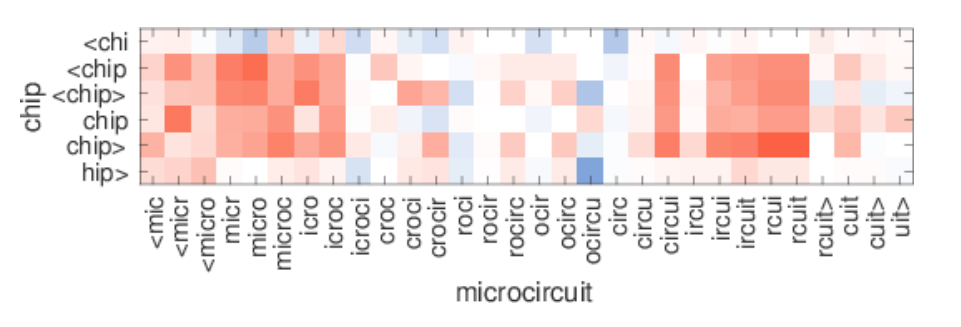
\includegraphics[width=0.7\textwidth]{fasttext_oov_similarity.png}
% 	\caption{Character n-gram similarity between the OOV word \enquote{microcircuit} and IV word \enquote{chip}. Positive and negative cosine similarity are denoted in red and blue respectively. Figure adapted from \cite{bojanowski2017}}
% 	\label{fig:fasttext_oov_similarity}
% \end{figure}

%TODO: conclusion to this section is needed: what follows that concerns the work you have done?
%TODO: Need to include disadvantages of fasttext to make a contrast
%\cite{bojanowski2017} report excellent training times for their unsupervised approach, without the need for any pre-processing, while outperforming other benchmark models that do not make use of sub-word information or use techniques such as morphological analysis.
\end{document}